\documentclass{article}
\usepackage{amsmath}
\usepackage{graphicx}

\title{Construction}
\date{Dec 2023}
\begin{document}
\maketitle
\begin{enumerate}
\item Draw a circle of radius $3.5cm$ .Take a point P outside the circle at a distance of $7cm$ from the center of the circle and construct a pair of tangents to the circle from that point.

\item Contruct a $\bigtriangleup ABC $ with sides $BC = 6cm$ ,$AB = 5cm$ and $\angle ABC = 60^{\circ}$ .Then construct a triangle whose sides are $\frac{3}{4}$ of the corresponding sides of $\bigtriangleup ABC$.

\item In Figure-1,$DE || BC $.If $\frac{AD}{DB}=\frac{3}{2}$ and $AE = 2.7cm$, then $EC$ is equal to
	(A) $2.0cm$ \newline
	(B) $1.8cm$ \newline
	(C) $4.0cm$ \newline
	(D) $2.7cm$ \newline
	
	\begin{figure}[h]
		\centering
		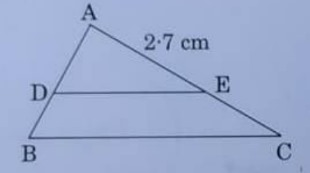
\includegraphics[width=\columnwidth]{figs/Construction.jpg}
		\caption{}
	\end{figure}

\item In Figure-2 ,if $PQ || BC$ and $PR || CD$ that $\frac{QB}{AQ} = \frac{DR}{AR}$.

\end{enumerate}
\end{document}
